\graphicspath{ {./images/} } % specify image path
\begin{center}
     \Large{2. Control}
\end{center}
\begin{itemize}
    \item \textbf{Denotational Semantics} formalises a language using semantic functions that map the language's components(syntatic domain) to mathematical objects(semantic domain) describing their behavior. 
    \item \textbf{Structural Operational Semantics} formalises program's execution by partitioning it into states and defining rules which determine the transition from one state to another. 
\end{itemize}

\begin{center}
     \textbf{Compilers and Interpreters}
\end{center}
\begin{itemize}
    \item \textbf{Interpreters} are written in their source language and used to execute programs written in a target language. (Runtime)
    \item \textbf{Compilers} are written in their source language and translate a program from a from-language to a to-language. (Compile Time)
    \item Needs to worry about recursion(usually not expanded) and scoping issues.
\end{itemize}
\begin{center}
    \begin{tabular}{ c c c c }
    \hline
    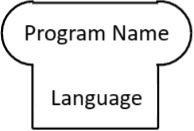
\includegraphics[scale=0.5]{images/t diagram program.jpg} & 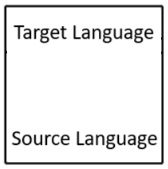
\includegraphics[scale=0.5]{images/t diagram interpreter.jpg} & 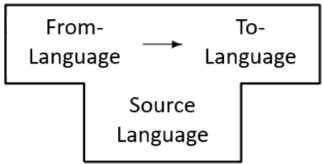
\includegraphics[scale=0.5]{images/t diagram compiler.jpg} & 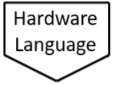
\includegraphics[scale=0.5]{images/t diagram hardware.jpg} \\
    \rowcolor{yellow}
    Program & Interpreter & Compiler & Hardware \\
    \hline
    \end{tabular}
\end{center}

\begin{center}
     \textbf{Modern Programming Languages}
\end{center}
\begin{itemize}
    \item Modern Languages desire lexical scoping, first-class functions(treated as a data type), variable assignment \& stateful data structures, automatic memory management, dynamic typing and statement oriented syntax(statements perform actions but may not return values).
    \item \textbf{Statement oriented syntax} is employed by imperative languages, where statements perform actions which change the state of the program. This can lead to unintended side effects.
    \item \textbf{Expression oriented syntax} is employed by functional languages, where all statements are expressions which return a value. This reduces unintended side effects as there is no program state.
    \item \textbf{Imperative Languages} have names which refer to locations, for which assignment destructively changes the stored value in the location. Statements are distinct from expressions, meaning returns are explicit and can appear anywhere in a function.
    \item \textbf{Functional Languages} do not have the assignment operation so names refer to values. All statements are expressions with return values, so returns are implicitly the result of evaluating the function's expression.
\end{itemize}

\begin{center}
     \textbf{CSE Machine (Control)}
\end{center}
\begin{itemize}
    \item Language agnostic model for explaining a program's execution by decomposing it into the following execution components and handling them accordingly.
    \item \textbf{Expression Nesting} is a basic control technique, processing it requires the decomposition of the expression into its basic, operable components. 
    \item \textbf{Sequential Composition} is sequentially assembling statements into a program, having the result/outcome of the previous statement feed into the next one. Use \code{pop} to remove the previous result from the stash if it is not needed.
    \item \textbf{Conditionals} allow branching in the control flow based on the evaluation of a predicate. Conditional statements can change code flow whilst conditional expressions change the returned value. \code{elif} is treated as a nested conditional.
    \item \textbf{Blocks} limits the scope of names within the block. When entering the block, we extend the current environment with bindings of all the names declared in the block. When exiting, we revert to the environment previously extended from with \code{env}. Execution in the block proceeds relative to the environment it creates.
    \item \textbf{Loops} repeat a certain section of code until the specified criteria is met. Each iteration extends a frame from the calling environment and exits it at the end of its execution.
    \item \textbf{Functions} are first class(treated like other data types). A function captures the environment it was defined in and extends from it during every subsequent call to the function.
    \item \textbf{Exceptions} are built into the language or thrown by the programmer to deviate the program's control flow to the latest "handler", which can then be chained.
\end{itemize}

\newpage

\begin{center}
     \textbf{Control Passing Styles}
\end{center}
\begin{itemize}
    \item \textbf{Continuation Passing Style} is a style of functional programming requires the explicit passing of control in the form of a continuation. Functions in this style take in an additional parameter known as the continuation, a function that takes in 1 argument. The continuation is the state of execution right before the function call. When the function finishes its execution, it calls the continuation with its result variable, which essentially treats that result variable as the return value from the function and continues with code execution.
    \item \textbf{Direct Style} is the common method to control passing, juxtaposed to the continuation passing style. It uses implicit and explicit returns which automatically return the execution state to when the function is called with the function's return value.
\end{itemize}

\begin{center}
     \textbf{Tail Recursion}
\end{center}
    Tail recursion occurs when recursion is the last operation in a function call. If there no variables declared in the function parameters and/or body need to be kept, compilers can optimise such recursive functions by reusing the stack frame for the next iteration. This essentially turns the recursion into an iteration and prevents stack overflow issues.